\section{Steganalysis}$First draft$
\label{steganalysis}
Steganalysis is the study of detecting information hidden with steganography and if possible, recover that information.
Because of the nature of steganography, it is not always obvious if a file has hidden information or not.
Therefore steganalysis is often used on a large set of files, which are suspected of containing hidden data.
%TODO: add more to intro

\subsection{Detection}
Most steganography algorithms are able to hide data without any notable visual impact on images.
It is therefore hard if not impossible to detect if something is hidden by simply looking at the image.

Detection of hidden data is therefore done with statistical tools like looking at histograms, modified DCT coefficients and signatures of different steganography algorithms.

\paragraph*{Colour Histogram}
A colour histogram is a representation of the distribution of colours in an image. 
This can be used to detect unusual distributions of colour, which may occur when using modifying the least significant bit or bits of each colour channel.

We have our cover image \ref{fig:CoverImage} and its respective colour histogram in figure \ref{fig:HistoWithoutLSB}.
We then hide another image in our cover image, this produces a new colour histogram (figure \ref{fig:HistoWithLSB}).
The new stego image has quite an unusual histogram, though sadly we cannot be sure there is hidden data only by looking at these histogram.

This unusual histogram might just be a product of a compression algorithm.

\paragraph*{DCT coefficients histogram}
By looking at a histogram of the DCT coefficients of a JPEG image, one might be able to detect if data has been hidden.
This is because of steganography algorithms like F5, the ``shrinkage'' it uses will result in a high amount of zeros in the DCT coefficients.
If we predict the histogram of the original cover image and compare it to the histogram of suspected image.
To estimate the DCT coefficients of the original cover image, we need to crop the suspected image by 4 vertical columns and recompress it using the same quantization table. \ref{Fridrich2003}
%TODO: make histogram of DCT coefficients and add F5 to section "State of the art"

\paragraph*{}

\paragraph*{Steganography signatures}
Unusual patterns in a image are obvious and arise suspicion, for example unused bits in the file headers or even comment headers, these might give us some insight into which algorithm was used.

\subsection{Recovery}
Recovery of data hidden with steganography is difficult, to recover the data we must know what kind of algorithm was used to hide the data.
Even if we know the algorithm used, we might still only get back meaningless data, because in addition to hiding the data, it might also be encrypted.

So the most common way of recovering hidden data is by using the same algorithm that was used to encode the image to decode the data.

\begin{figure}
	\centering
	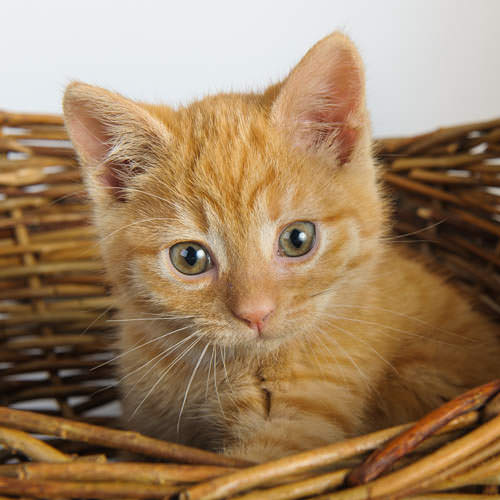
\includegraphics[width=0.5\textwidth]{figures/cover.jpg}
	\caption{Cover image.}
	\label{fig:CoverImage}
\end{figure}

\begin{figure}
	\centering
	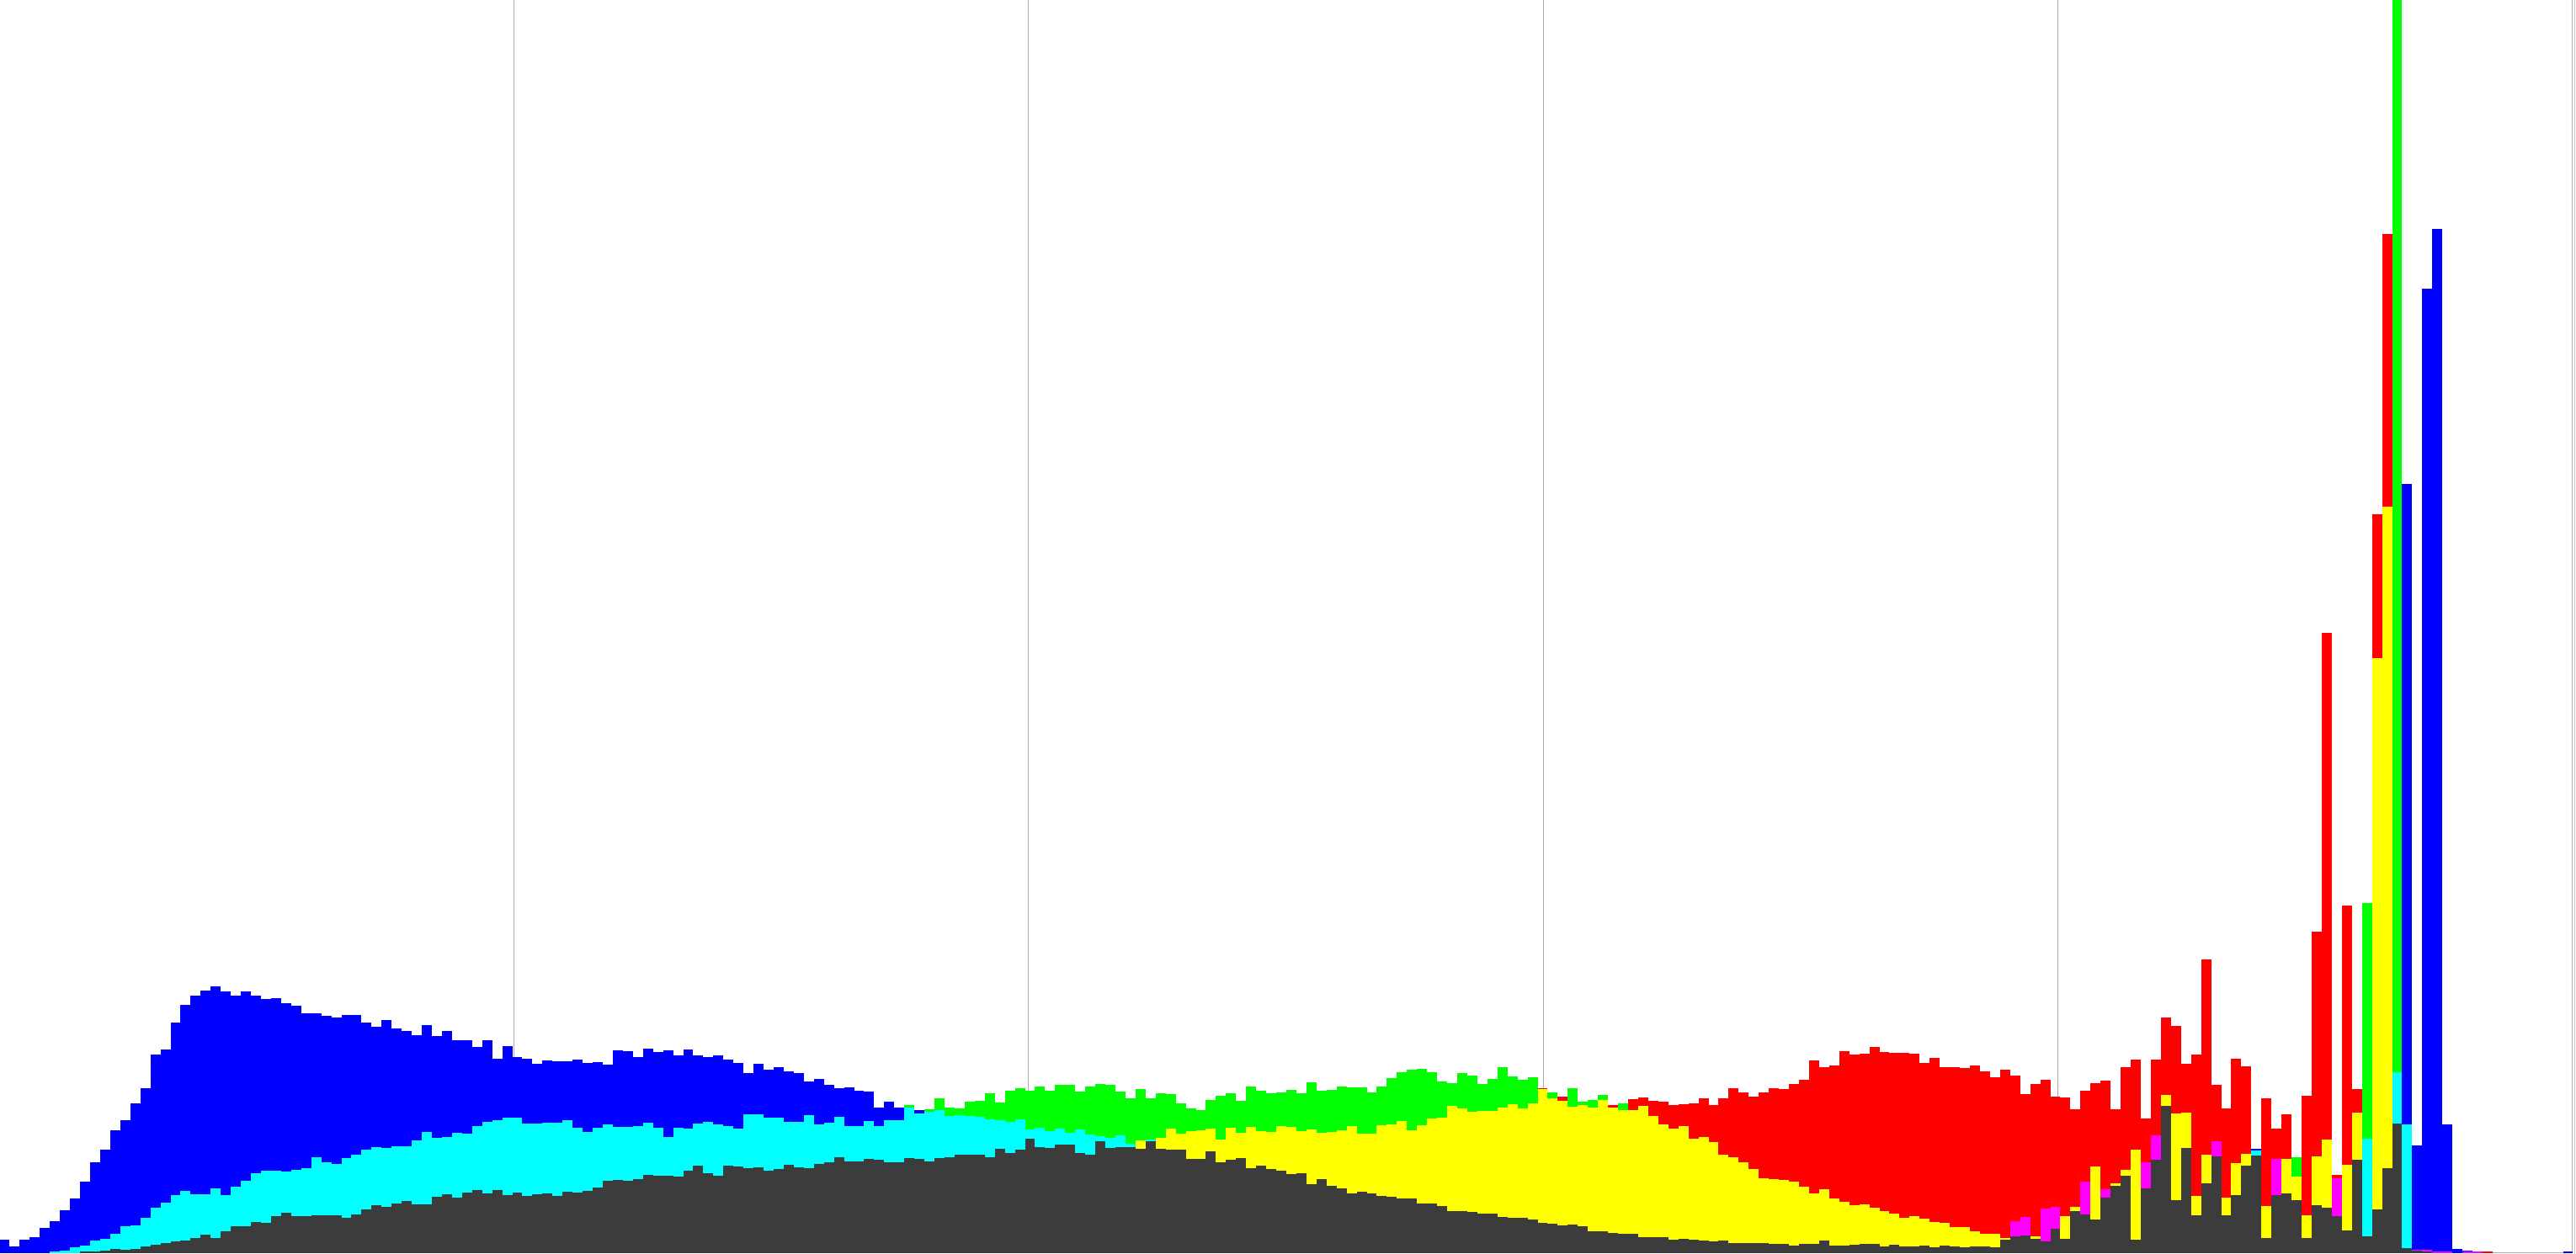
\includegraphics[width=1\textwidth]{figures/HistoLSBCat.png}
	\caption{Colour Histogram of image without hidden data.}
	\label{fig:HistoWithoutLSB}
\end{figure}

\begin{figure}
	\centering
	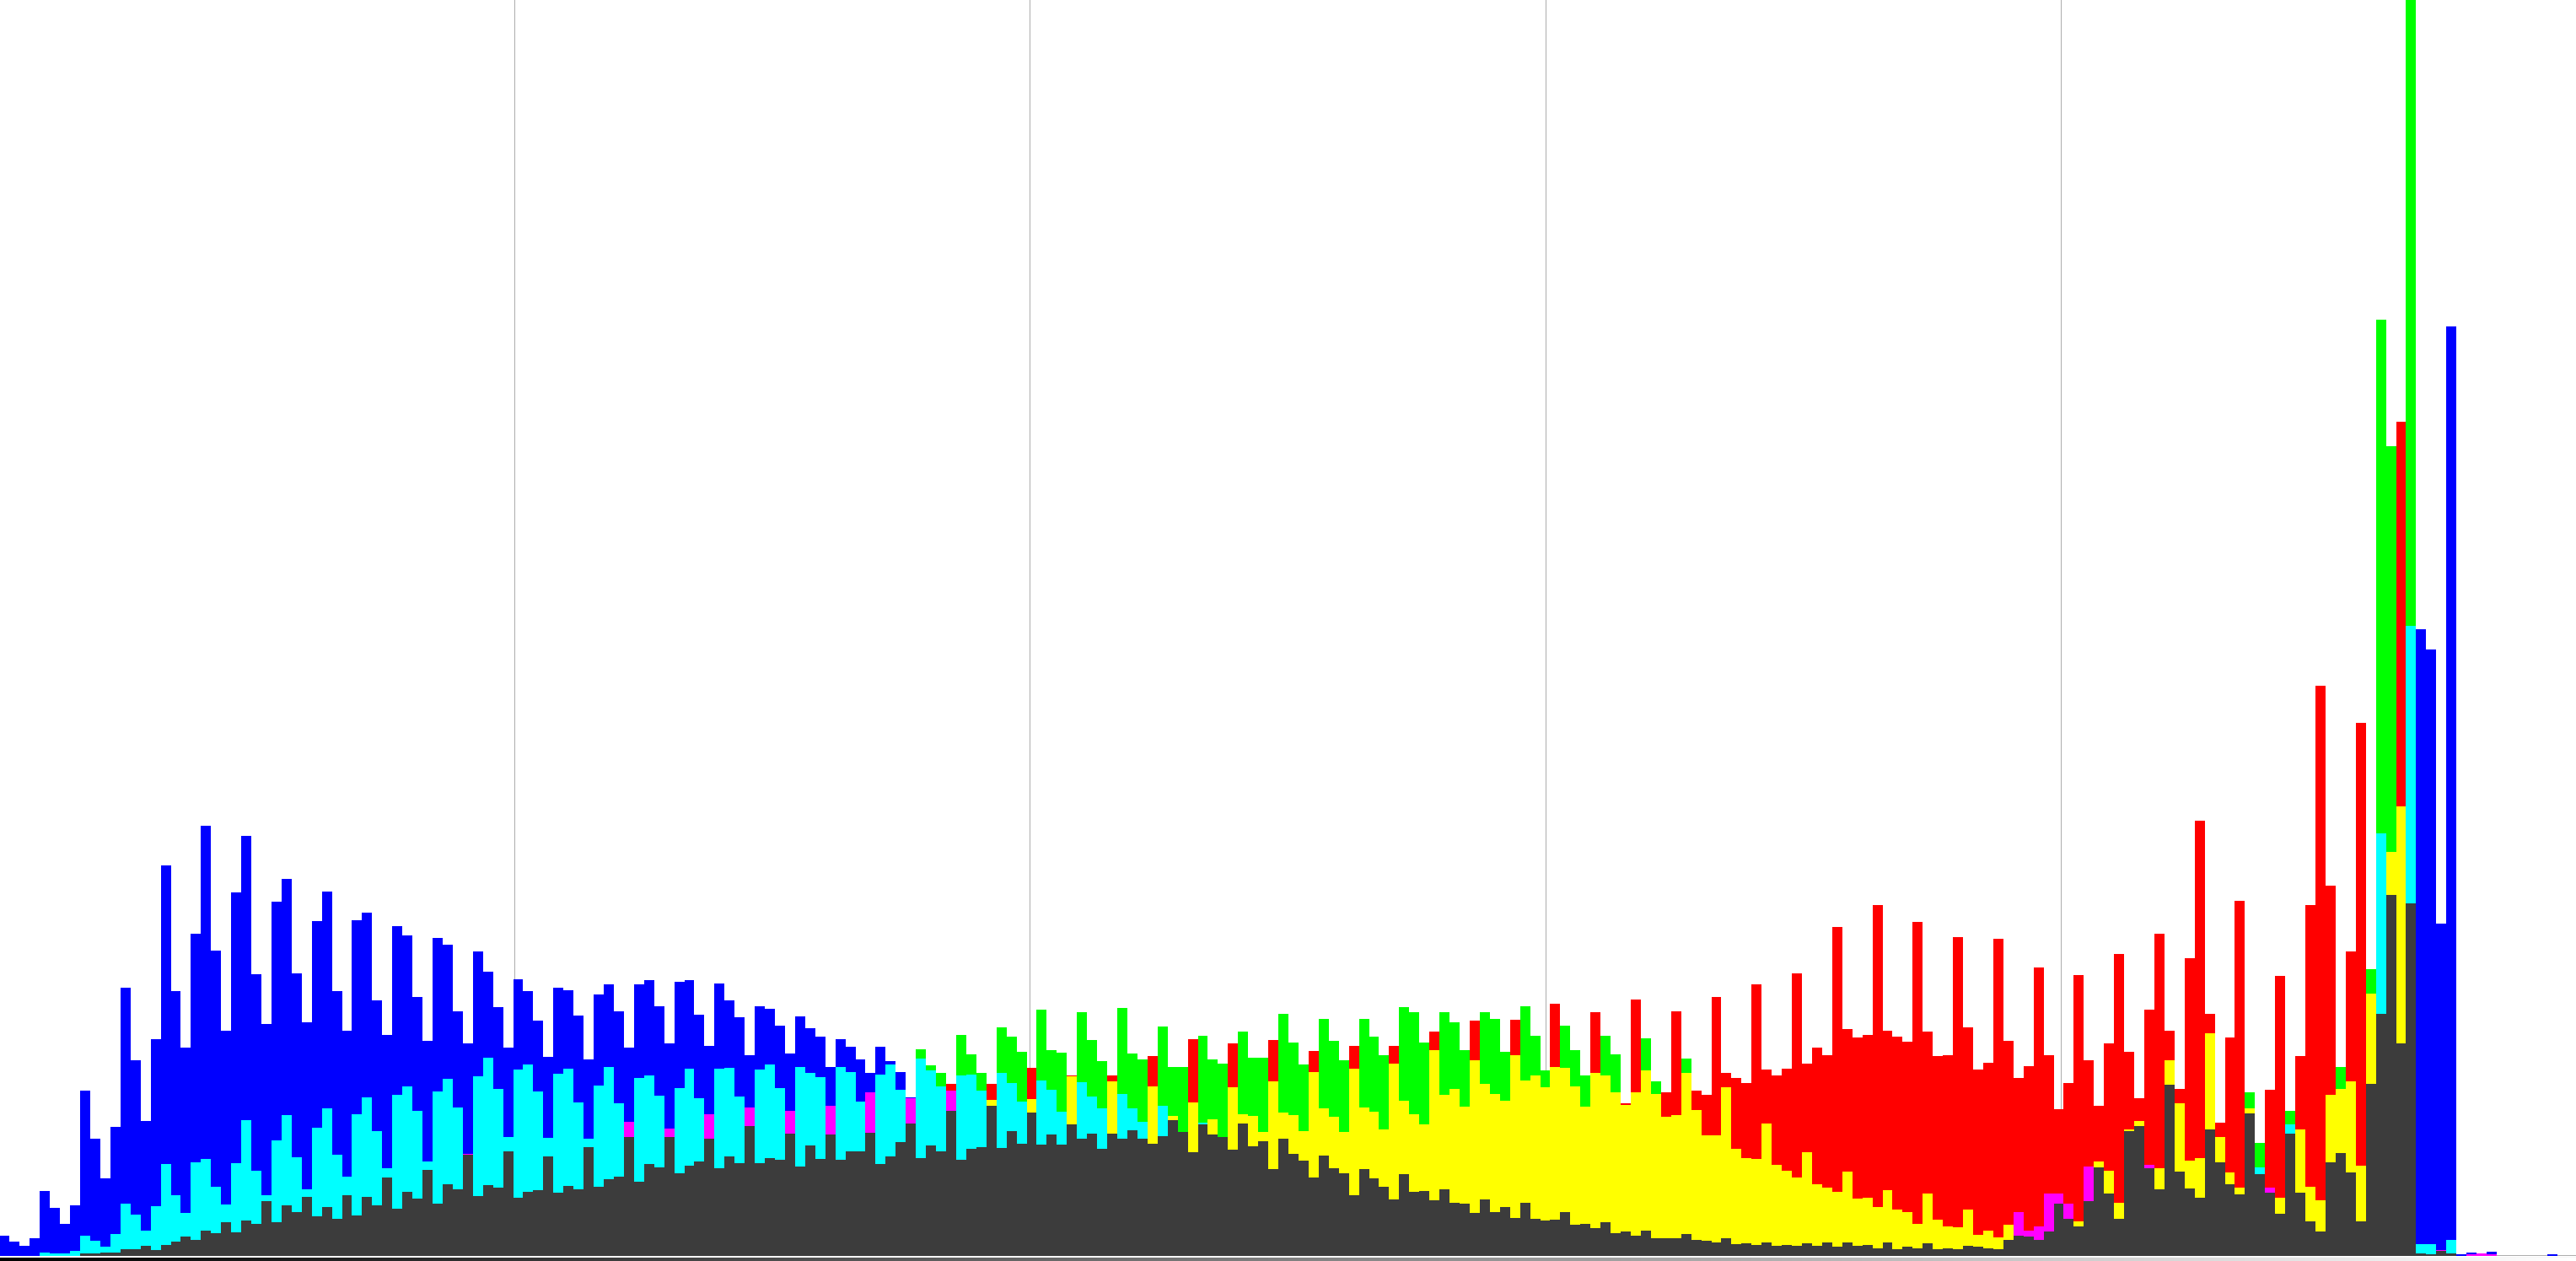
\includegraphics[width=1\textwidth]{figures/HistoLSBCatEncrypted.png}
	\caption{Colour Histogram of image containing secret image hidden with LSB.}
	\label{fig:HistoWithLSB}
\end{figure}
